\documentclass[8pt]{standalone}

\usepackage{tikz}
\usetikzlibrary{calc,positioning}

\begin{document}
	\begin{tikzpicture}
	
	\node[anchor = north west, inner sep=0] (360LF) at (0, 0) {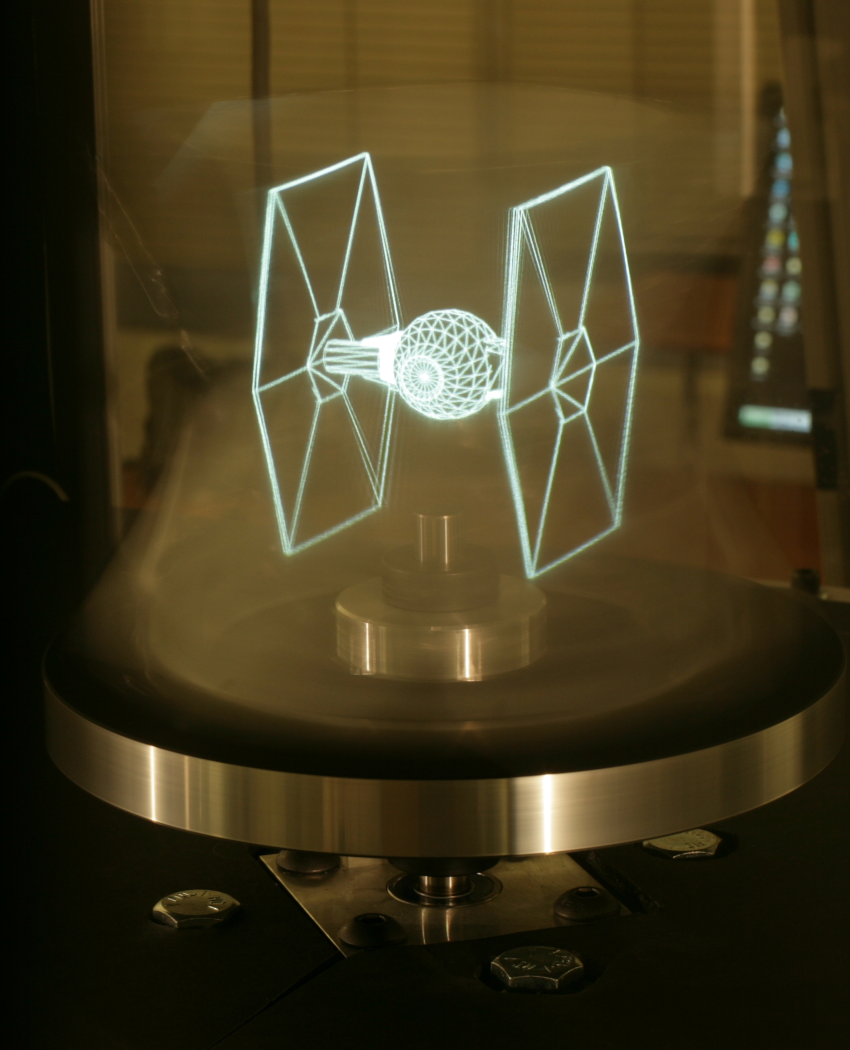
\includegraphics[height=10cm]{360_deg_display}};
	\node[align = center, below = 0.3cm of 360LF, inner sep = 0] {Jones et al. [2007]};
	
	\node[anchor = north west, inner sep=0, draw = black] (parallaxIntegral) at (10, 0) {\includegraphics[height=10cm]{parallax_barrier_vs_lenticular}};
	\node[align = center, below = 0.3cm of parallaxIntegral, inner sep = 0] {en.wikipedia.org/wiki/Autostereoscopy};
		
	\end{tikzpicture}	
\end{document}

%
%\begin{columns}
%		\column{0.33\textwidth}
%			
%			\\
%			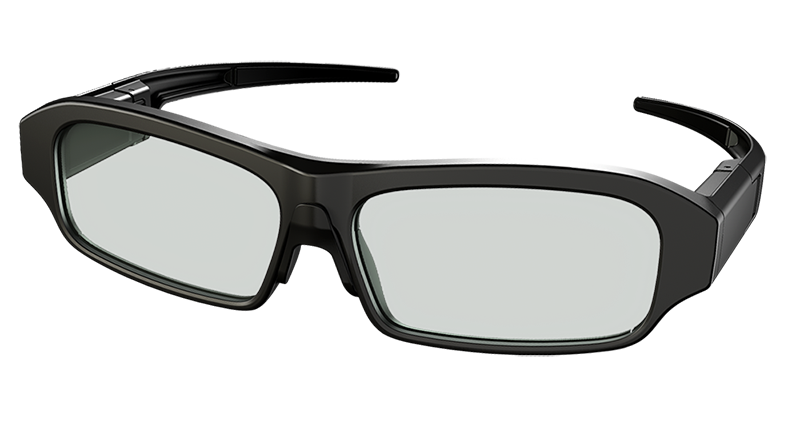
\includegraphics[width=3cm]{images/3d_glasses}
%		\column{0.33\textwidth}
%			Add more images
%		\column{0.33\textwidth}
%			\includegraphics[height=5cm]{images/parallax_barrier_vs_lenticular}
%\end{columns}